\nnarticleheader{Exploring Symmetry in Quantum Physics}{Brian Williams, Haverford '21}

\noindent
\textbf{Introduction}

Humanity has always been drawn to symmetry, both in nature and in the structures we build ourselves. Perhaps our brains are wired to see beauty in symmetry, or maybe we just find practicality in order. Regardless of our reasons for liking symmetry, it seems that nature itself has its own affinity for it. Some symmetries arise naturally from the laws governing our universe, and some seem to give rise to laws of their own---especially in quantum physics. 

But what exactly \emph{is} symmetry? What does it mean for a system to be symmetrical? Well, an object has a symmetry if when you do something to it---move it, turn it, flip it---it looks the same after you're done with it. For example, a butterfly looks symmetrical because when you reflect it across its $y$-axis, it's hard to tell that anything has changed. More specifically, it has a particular \emph{symmetry corresponding to that transformation}.

As a more detailed example, consider a hydrogen atom, a system with just a proton and an electron. The proton is much heavier than the electron, so we really only need to consider the electrostatic potential on the latter, which generates a force that pulls the electron towards the proton. The potential energy is inversely proportional to the distance between the two particles, meaning that we can write it as $V(r)$, where $r = \sqrt{x^2 + y^2 + z^2}$, as opposed to $V(x, y, z)$. This property gives rise to an interesting symmetry of the system: if we rotate the electron around the origin, the value of the potential shouldn't change. After all, it only depends on the distance to the origin. For instance, a $90^{\circ}$ rotation around the $z$-axis involves the substitutions
\begin{align*}
    x &\rightarrow -y \\
    y &\rightarrow x \\
    p_x &\rightarrow -p_y \\
    p_y &\rightarrow p_x
\end{align*}
where $x$, $y$, and $z$ are the position variables, and $p_x$, $p_y$, and $p_z$ are the momentum variables (since we rotated around the $z$-axis, $z$ and $p_z$ are left unchanged):
\begin{align*}
    r &= \sqrt{(-y)^2 + (x)^2 + z^2} \\
    &= \sqrt{x^2 + y^2 + z^2}.
\end{align*}
Its form is unchanged---and you would find the same with any other rotation around the origin. In other words, the system has some sort of rotational symmetry.

But what about the changes in $p_x$ and $p_y$? Since we looked at the potential energy, we might as well do the same to the kinetic energy
\begin{align*}
    T = \frac{p_x^2 + p_y^2 + p_z^2}{2m}
\end{align*}
which upon plugging in the two momentum variable substitutions we didn't use before, we find is also invariant. By contrast, if we'd had a transformation like $p_x \rightarrow 0$, then there would be a clear difference in the behavior between the original and transformed systems. So in order to analyze the effect of a transformation on a system, we need to consider both the kinetic energy $T$ and potential energy $V$. Here's one useful way to do this, using an object called the \emph{Hamiltonian}:
\begin{align*}
    \mathscr{H} = T + V.
\end{align*}
It's really just a fancy name for the sum of the total kinetic and potential energy. Despite its seemingly simple form, it contains all the information about how a system behaves, or changes over time.\footnote{Classically, one can use a set of equations called the \emph{canonical equations} to do this. This is called the \emph{Hamiltonian formalism}, as opposed to the Newtonian approach which uses Newton's three laws, including $F = ma$, to figure out how a system behaves.} So here's the key point: when a transformation leaves the Hamiltonian invariant, the \emph{behavior of the system} is left invariant.

\noindent
\textbf{Transformations in Quantum Mechanics}

In order to examine transformations in quantum mechanics---which are a bit more abstract than just substituting variables---we'll need some notation. Let $A$ be some abstract transformation, which we could apply to some abstract object represented by the symbol $|v\rangle$ (pronounced ``ket v''). For example, $A$ could be the rotation of some object by 90 degrees (about the $z$-axis) and $|v\rangle$ could be the butterfly we were talking about before. After being acted upon by the rotation $A$, the butterfly will end up in a new rotated state $|v'\rangle$:
\begin{center}
    \centering
    \begin{minipage}{0.4\textwidth}
        \centering
        \begin{tikzpicture}
            \draw[black, thin] (-0.4\textwidth,0) -- (0.4\textwidth,0);
            \draw[black, thin] (0,-0.4\textwidth) -- (0,0.4\textwidth);
            \node (butterfly) at (0,-0.035\textwidth) 
            {
\includegraphics[width=.45\textwidth]{williams_butterfly.png}};
            \node (ket) at (0.25\textwidth, 0.25\textwidth) {$|v\rangle$};
        \end{tikzpicture}
    \end{minipage}
    \begin{minipage}{0.1\textwidth}
        \centering
        \begin{tikzpicture}
            \draw[black, thick, ->] (-0.5,0) -- (0.5,0);
            \node at (0, 0.3) {$A$};
            \node at (0, -0.4) {};
        \end{tikzpicture}
    \end{minipage}
    \begin{minipage}{0.4\textwidth}
        \centering
        \begin{tikzpicture}
            \draw[black, thin] (-0.4\textwidth,0) -- (0.4\textwidth,0);
            \draw[black, thin] (0,-0.4\textwidth) -- (0,0.4\textwidth);
            \node (butterfly) at (0.03\textwidth,0)
            {
\includegraphics[width=.45\textwidth, angle=90]{williams_butterfly.png}};
            \node (ket) at (0.25\textwidth, 0.25\textwidth) {$|v'\rangle$};
        \end{tikzpicture}
    \end{minipage}
\end{center}
To show this relation, we write
\begin{align*}
    A|v\rangle = |v'\rangle.
\end{align*}

This bracket-based notation, quite imaginatively called bra-ket notation, is common in quantum mechanics.\footnote{I might as well add that there's another symbol called a ``bra'' which looks like $\langle v|$. If you're familiar with linear algebra, $\langle v|$ is the conjugate transpose of $|v\rangle$.} We haven't really defined what $A$ and $|v\rangle$ mean mathematically, but for these purposes it's probably better to think of them just in terms of what they represent: a transformation and an object being transformed. Formally, $A$ is called an \emph{operator} and $|v\rangle$ is actually a \emph{vector}.\footnote{But try not to think of $|v\rangle$ as a vector like an arrow in space, like you usually do.} In quantum mechanics, a \emph{statevector} like $|v\rangle$ or $|\psi\rangle$ represents a particular state of the system (the Greek letter $\psi$ ``psi'' is most commonly used for some arbitrary state). For example, $|\psi_0\rangle$ could represent an electron bound to a proton, while $|\psi_1\rangle$ could represent the same electron that just got released some time later.

Before moving on, I'd like to emphasize the difference between the dynamics of a system and a particular state of a system. When we considered the rotation of the hydrogen atom, we looked at a symmetry of the \emph{dynamics} of the system. The Hamiltonian didn't change, so the electron still moves in the same way we'd expect. But (if we imagine the electron as a classical particle with definite position) the position of the electron still changed after the rotation. In quantum mechanics, the dynamics of the whole system itself are represented by some Hamiltonian \emph{operator} $H$, similar in structure to the Hamiltonian function $\mathscr{H}$ we looked at before. An isolated hydrogen atom has some particular $H$ which dictates how the system changes over time. On the other hand, the state of the system $|\psi\rangle$ will change over time depending on $H$. As we will see, however, we can look at how a statevector is affected by transformations to reveal transformations regarding the dynamics of the whole system.

Now we have the tools we need to analyze transformations in quantum mechanics. Some examples of transformations you've probably seen are spatial translations, rotations, and reflections, as mentioned above. We can use specific operators for these, like $T(\mathbf{a})$ (to translate the state by the vector $\mathbf{a}$), $R_x(\theta)$ (for a rotation by $\theta$ around the $x$-axis), and $\Pi$, respectively. The $\Pi$ operation is commonly called a \emph{parity} transformation. Here's an example of what a translation operator would look like for a one-dimensional system, where we only consider the $x$-direction:
\begin{align*}
    T(a)|x\rangle = |x+a\rangle
\end{align*}
where $|x\rangle$ is a state with a well-defined position at $x$. Classically, this would mean doing
\begin{align*}
    x \rightarrow x+a.
\end{align*}
To describe a series of transformations, let's say a translation first and then a rotation, we would write $R_x(\theta)T(\mathbf{a})|\psi\rangle$, where the operators closest to $|\psi\rangle$ act first.

We can also consider transformations involving time, such as moving forward or backwards in time $U(t)$---we'll call this \emph{time evolution}---or reversing time similar to the parity transformation ($t \rightarrow -t$), called \emph{time-reversal}. To represent a state at time $t=0$, we write $|\psi(0)\rangle$
\begin{align*}
    U(t)|\psi(0)\rangle = |\psi(t)\rangle
\end{align*}

The operators $H$ and $U(t)$ are very closely related---as mentioned before, the Hamiltonian contains the information about how a system behaves, so it makes sense that it'd be tied to an operator $U(t)$ that moves the system forwards in time. It's pretty common to be given a Hamiltonian and use it to find $U(t)$, in the same way that you might be given the forces or potentials in a classical system and use Newton's laws to find the equations of motion.

Consider the symmetries coming from these transformations. The translation, rotation, and time evolution operators are controlled by a specific parameter, meaning that they are \emph{continuous}. You can choose how much you'd like to move, rotate, or evolve a state. By contrast, the parity and time-reversal transformations are \emph{discrete}. We saw that our mirrored butterfly had a discrete symmetry. What about the hydrogen atom? Well, since it didn't matter how much we rotated it, it seems to have a continuous symmetry.

Now that we have this notation, there's a much easier way to write that a system with a Hamiltonian $H$ has a certain symmetry, let's say under a transformation $A$. Let's say we have a state $|\psi\rangle(0)$ at time $t=0$ and let it change over time. This change depends on $U(t)$, which in turn depends on the Hamiltonian $H$:
\begin{align*}
    U(t)|\psi(0)\rangle = |\psi(t)\rangle.
\end{align*}
Now let's imagine a different scenario, where we had transformed our state according to $A$ at $t=0$ and \emph{then} let it change over time:
\begin{align*}
    U(t)A|\psi(0)\rangle = A|\psi(t)\rangle.
\end{align*}
Since the system is symmetrical under $A$, there shouldn't be any difference in how the states changed over time---the system still behaves in the same way. In other words, the two end results, $U(t)|\psi(0)\rangle$ and $U(t)A|\psi(0)\rangle$, should only differ by a transformation on the former:
\begin{align*}
    AU(t)|\psi(0)\rangle = U(t)A|\psi(0)\rangle.
\end{align*}
But since this is a symmetry of the system, not this particular state, we only need to write
\begin{align*}
    AU(t) = U(t)A
\end{align*}
to mean that our system has a symmetry corresponding to $A$.

Although it might be tempting to think that $AU(t) = U(t)A$ no matter the scenario, this isn't always the case. All natural laws, like the electromagnetic, weak nuclear, and strong nuclear forces, are invariant under space and time translations. The weak force, however, isn't invariant under parity transformations. This force is responsible for radioactive beta decay. In 1956, physicist Chien-Shiung Wu performed an experiment with the following beta decay in cobalt-60:
\begin{align*}
    ^{60}\text{Co} \rightarrow\: ^{60}\text{Ni} + e^- + \Bar{\nu}
\end{align*}
where $e^-$ is an electron and $\Bar{\nu}$ is an antineutrino. She found that the electrons had a preferred direction in which they'd decay, opposite the spin $^{60}\text{Co}$, leading to the conclusion that parity symmetry was \emph{violated}. So although this is a situation in which there's a lack of symmetry, this actually helps us understand the universe better---nature treats a completely mirrored version of the universe differently than a non-mirrored one, contrary to what you might expect.

\noindent
\textbf{Conservation Laws}

In 1918, mathematician Emmy Noether proved a theorem linking continuous symmetries to \emph{conserved quantities}. A conserved quantity is one that doesn't change over time---for example, if the momentum of a system is conserved, then the system should have the same momentum after waiting for a little while:
\begin{align*}
    \frac{dp}{dt} = 0.
\end{align*}
This theorem, which applies to both classical and quantum systems, is extremely important in explaining the correspondence between the symmetries and behaviors of a system.
\begin{theorem}[Noether's theorem]
Every continuous symmetry in a system corresponds to a conserved quantity.
\end{theorem}
Here are the relationships from the continuous symmetries we've looked at:
\begin{center}
    \begin{tabular}{|c|c|c|}
    \hline
    Transformation & Operator & Conserved quantity \\
    \hline
    Translation & $T$ & Momentum \\
    Rotation & $R$ & Angular momentum \\
    Time evolution & $U$ & Energy \\
    \hline
    \end{tabular}
\end{center}
The first two might look like they make sense, but the third isn't immediately obvious. But remember that the Hamiltonian---the total energy of the system---dictates the behavior of the system over time.

Since our hydrogen atom had rotational symmetry, we can use Noether's theorem to reason that if the system isn't tampered with, the angular momentum of a state shouldn't change over time. This is a nice way to skip some calculations, but it's also possible to go the other way: it's possible to take a variable, like position or energy, and derive, or \emph{generate} a transformation operator from it. Variables in quantum mechanics like position and momentum also happen to be represented by operators, such as $X$ and $P$, which can be used to generate the translation and rotation operators. We won't go into the details since that gets into some technical linear algebra, but just knowing the relationship between symmetries and conserved quantities is a key part of understanding symmetries in quantum mechanics and physics in general.

\noindent
\textbf{Energy Levels}

For a system with a Hamiltonian $H$, there are certain states $|E\rangle$ with definite energies $E$:
\begin{align*}
    H|E\rangle = E|E\rangle
\end{align*}
where $E$ is a number (but $H$ is an operator, like before). In general, a system could have discrete or continuous energy levels, or possibly both. From chemistry, for example, you'll remember that the electrons in an atom can occupy different discrete energy levels, and that photons can excite them to higher levels. The above equation can be solved to find these specific energies and states, but sometimes the Hamiltonian for a system can be extremely complicated---even for a helium atom, there are no exact solutions for $|E\rangle$. Instead, physicists must use approximations.

One common approach is to write the Hamiltonian as a sum of terms:
\begin{align*}
    H = H_0 + H_p.
\end{align*}
Remember that the Hamiltonian is just the kinetic plus the potential energy, so adding two Hamiltonians together just means introducing more kinetic or potential energy terms to our system (but an added Hamiltonian doesn't have to include another kinetic/potential term if we already have it included). If we wanted to analyze the helium atom, we could use $H_0$ to represent the attraction of the electrons towards the nucleus and $H_p$ for the electron-electron interaction. In general, $H_p$ could either be an approximation to the system we'd be trying to solve, or a physical external change to our system, like if we turned on a small magnetic field to disturb the atom, since this would introduce a new potential.

Here's where symmetry properties come into play: we can use them to figure out \emph{how the energy levels split} when we apply this $H_p$ term, called a $perturbation$. Let's say we have a system with multiple states $|E_1\rangle$ and $|E_2\rangle$ that correspond to the same energy $E$; these states are known as \emph{degenerate}. But it's possible that if we apply a perturbation---which could be us making a mathematical change to fix an approximation, or us actually applying some physical change like a magnetic field---these states in the same energy level might \emph{split} into states each with different energy levels.

When a Hamiltonian is symmetrical under a bunch of related transformations, like the hydrogen atom with any rotation around the origin, it's helpful to classify the set of all the transformations as an object called a \emph{group}. If you imagine rotating an object like a basketball, notice that a series of rotations in succession is always equivalent to some other, single rotation. Also notice that there's always an inverse transformation, namely a rotation that can bring the basketball from a rotated state back to where it was. In order for a set of transformations to be considered a group, it must satisfy those properties (two transformations from the group can be expressed as just one, there always exists an inverse transformation) and more. The group we just gave has an infinite amount of elements, since there are an infinite amount of rotations you could do, but there are also finite groups. Lots of molecules can be flipped or rotated in certain ways and look the same, but not in an infinite amount of ways, like a water or ammonia molecule.

\begin{wrapfigure}{r}{0.25\textwidth}
    \centering
    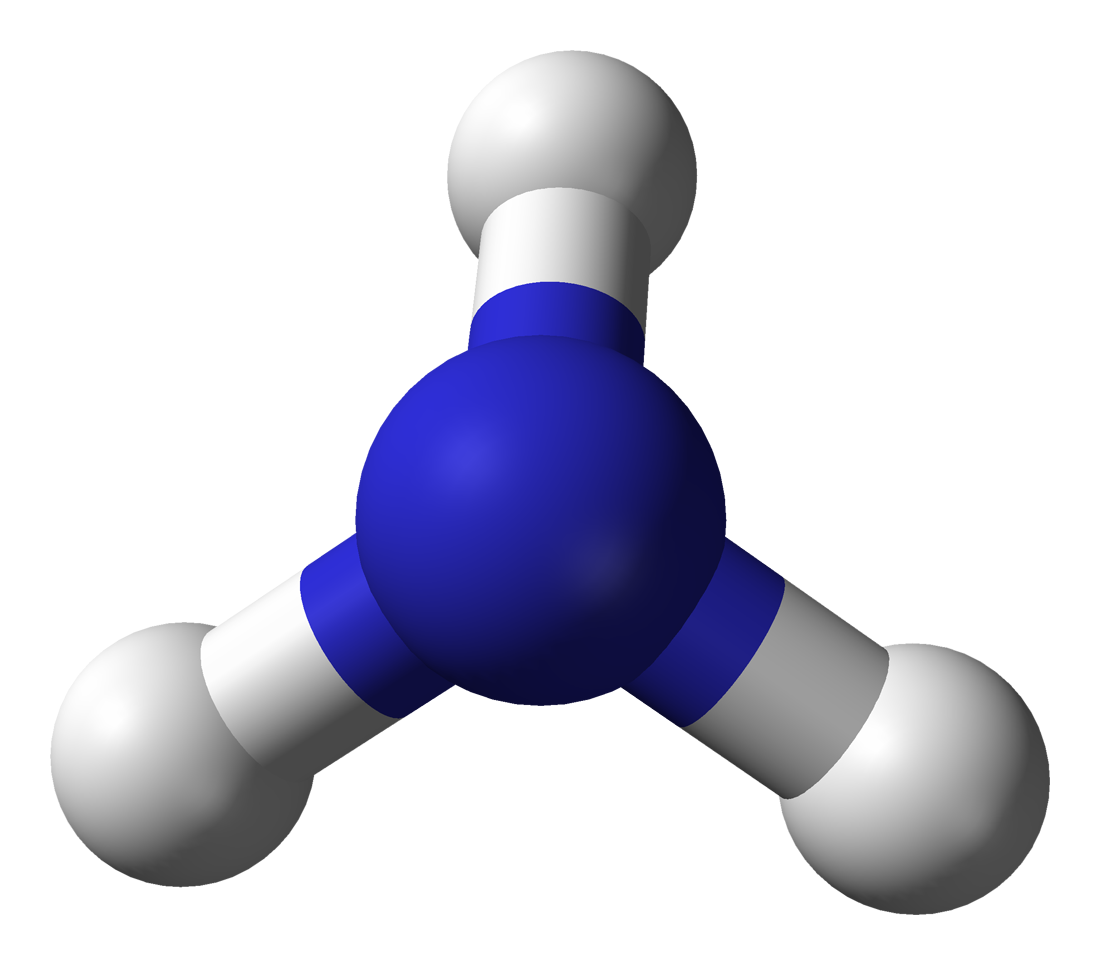
\includegraphics[width=0.2\textwidth]{williams_ammonia.png}
\end{wrapfigure}

It turns out that if a Hamiltonian is symmetrical under a certain group, then all of the states corresponding to one energy level are related to this group through a specific set of matrices, known as a \emph{representation} of the group. By knowing that set of matrices, not only do you have a way to figure out which states might belong to the same energy level, but it's also possible to figure out how much that energy level might split after a perturbation.

\noindent
\textbf{Conclusion}

A lot of the topics here (groups, Hamiltonian mechanics, conservation laws) could be discussed for much longer on their own, but the goal was to give an introduction to the roles they each play in understanding symmetry in quantum mechanics. Groups play a significant role in many aspects of quantum physics from the structure of molecules to the way the operators representing variables behave with each other. They play an even larger role in quantum field theory, to the point where the Standard Model---the theory of elementary particles including the electromagnetic, weak, and strong forces---can be described using a special symmetry group. 

Symmetry laws are valuable because---in contrast to approximations---the information we can derive from knowing the symmetries is \emph{exact}. Understanding symmetry, both in everyday life and in quantum mechanics, can make objects much easier to understand. Symmetries can also help us figure out the underlying laws dictating our world---though as we saw before with Wu's Cobalt-60 experiment, some symmetries can be broken. Interestingly, a theorem called the CPT theorem says that under simultaneous charge conjugation (switching all particles with their antiparticles), parity, and time-reversal, the laws of our universe \emph{shouldn't} change.

Once you've gotten a feel for the role that symmetries play in physics, it's really a matter of wondering why all of these symmetries exist, and why they're so appealing. Artists and architects often use symmetry to guide their works. Physicists often use symmetry to discover the laws governing our world. But do these symmetries appear by chance, emerging out of pure convenience? Or does nature itself, with its most fundamental laws, see the beauty in symmetry?


\begin{thebibliography}{2}

\bibitem{} 
Heine, Volker, and D.T. Haar. Group Theory in Quantum Mechanics: An Introduction to Its Present Usage. Elsevier Science, 2014. 

\bibitem{}
Shankar, Ramamurti. Principles of Quantum Mechanics. Springer, 1994.

\end{thebibliography}
